%================================================================================================
%================================= PRIMEIRA FOLHA INTERNA  ======================================
%================================================================================================

%\thispagestyle{empty} %Tirando o numero da primeira p�gina

\includegraphics [width=2cm] {unicamp.eps}

\vspace*{2.0cm}

\begin{center}
\large TIAGO DE FREITAS PEREIRA
\end{center}

\vspace*{3cm}

\begin{center}
{\sc ``A COMPARATIVE STUDY OF COUNTERMEASURES TO DETECT SPOOFING ATTACKS IN FACE AUTHENTICATION SYSTEMS"}
\\[1in]
{\sc ``UM ESTUDO COMPARATIVO DE CONTRAMEDIDAS PARA DETECTAR ATAQUES DE SPOOFING EM SISTEMAS DE AUTENTICA��O DE  FACES"}
\end{center}

\vspace*{3.25cm}

\null \vfill

\begin{center}
CAMPINAS\\2013
\end{center}



% parte de tr�s da primeira folha interna fica em branco
\newpage
\null \vfill
\thispagestyle{empty} %Tirando o numero da primeira p�gina
\newpage
\addtocounter{page}{-1}
%================================================================================================
%====================================== FOLHA DE ROSTO ==========================================
%================================================================================================

\includegraphics [width=2cm] {unicamp.eps}

\begin{flushleft}
\large \hspace*{2.5cm} UNIVERSIDADE ESTADUAL DE CAMPINAS\\
          \hspace*{2.5cm} Faculdade de Engenharia El�trica e de Computa��o
\end{flushleft}

\vspace*{1cm}
\begin{center}
\large TIAGO DE FREITAS PEREIRA
\end{center}

\vspace*{0.5cm}

\begin{center}
{\sc ``A COMPARATIVE STUDY OF COUNTERMEASURES TO DETECT SPOOFING ATTACKS IN FACE AUTHENTICATION SYSTEMS"}
\\[0.5in]
{\sc ``UM ESTUDO COMPARATIVO DE CONTRAMEDIDAS PARA DETECTAR ATAQUES DE SPOOFING EM SISTEMAS DE AUTENTICA��O DE FACES"}


\end{center}

\vspace*{0.5cm}

\begin{flushright}
\begin{minipage}{9.0cm}

Masters dissertation presented at the School of Electrical and Computer Engineering in partial fulfillment of the requirements for masters degree in Electrical Engineering. Concentration Area: Computer Engineering 
\\[0.2in]
Disserta��o de Mestrado apresentada na Faculdade de Engenharia El�trica e de Computa��o como  parte dos
requisitos exigidos para a obten��o do t�tulo de Mestre em Engenharia El�trica. �rea de
concentra��o: Engenharia de Computa��o

\end{minipage}
\end{flushright}

\null \vfill
\begin{minipage}{15cm}
Orientador: Prof. Dr. JOS� MARIO DE MARTINO
\vspace*{0.7cm}
\end{minipage}

\begin{minipage}{7cm}
\small
Este exemplar corresponde a vers�o final da disserta��o de mestrado apresentado pelo
aluno, e orientado pelo Prof. Dr. Jos� Mario De Martino\\[4mm]
\rule{7.0cm}{0.2mm} \hfill
\end{minipage}

\vspace*{0.5cm}

\begin{center}
CAMPINAS\\2013
\end{center}


%%%%%
%NEW BLANK PAGE
\newpage
\null \vfill
\thispagestyle{empty} %Tirando o numero da primeira p�gina
\addtocounter{page}{-1}


\newpage
%FICHA CATALOGRAFICA
%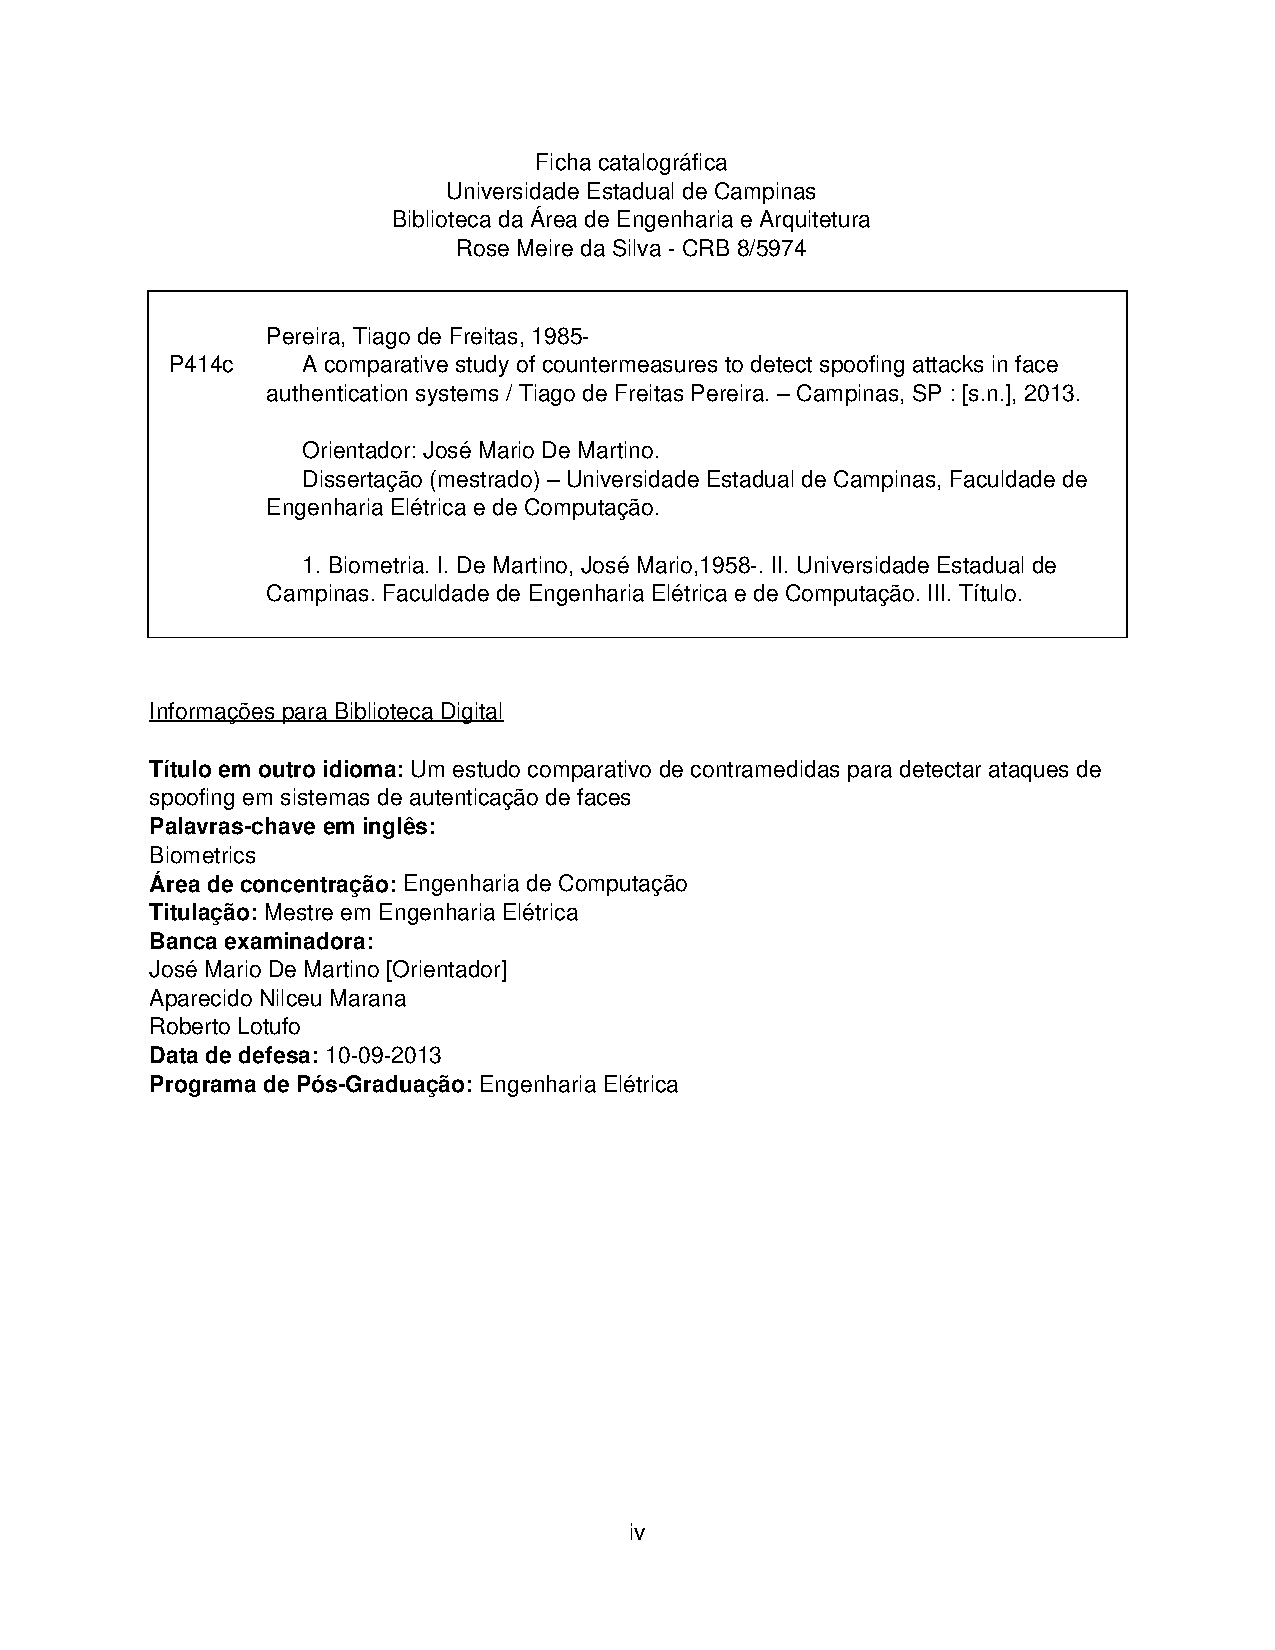
\includepdf[pages=-,pagecommand=\thispagestyle{plain} ,scale=1]{docs/Ficha-Catalografica-Protocolo-1355789.pdf}
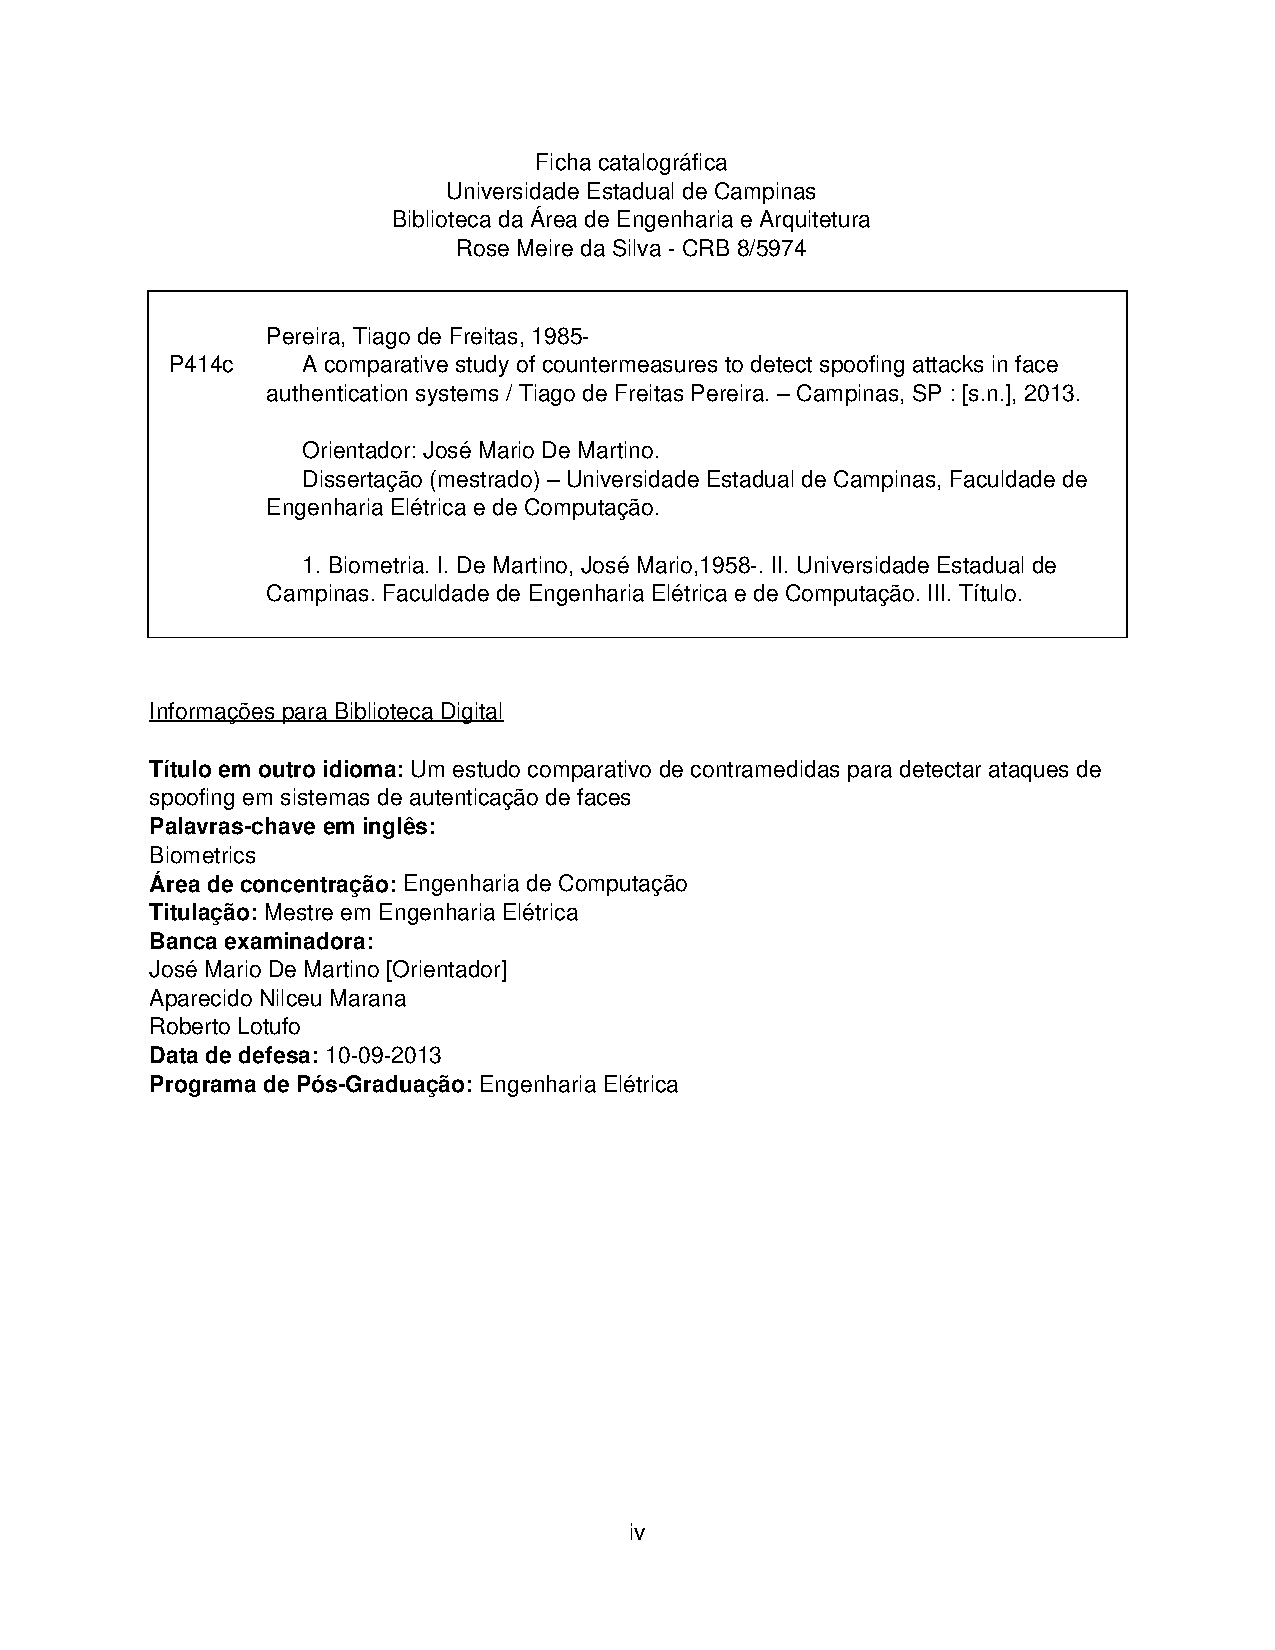
\includepdf[scale=1.09]{docs/Ficha-Catalografica-Protocolo-1355789.pdf}


%\newpage
%comissao julgadora
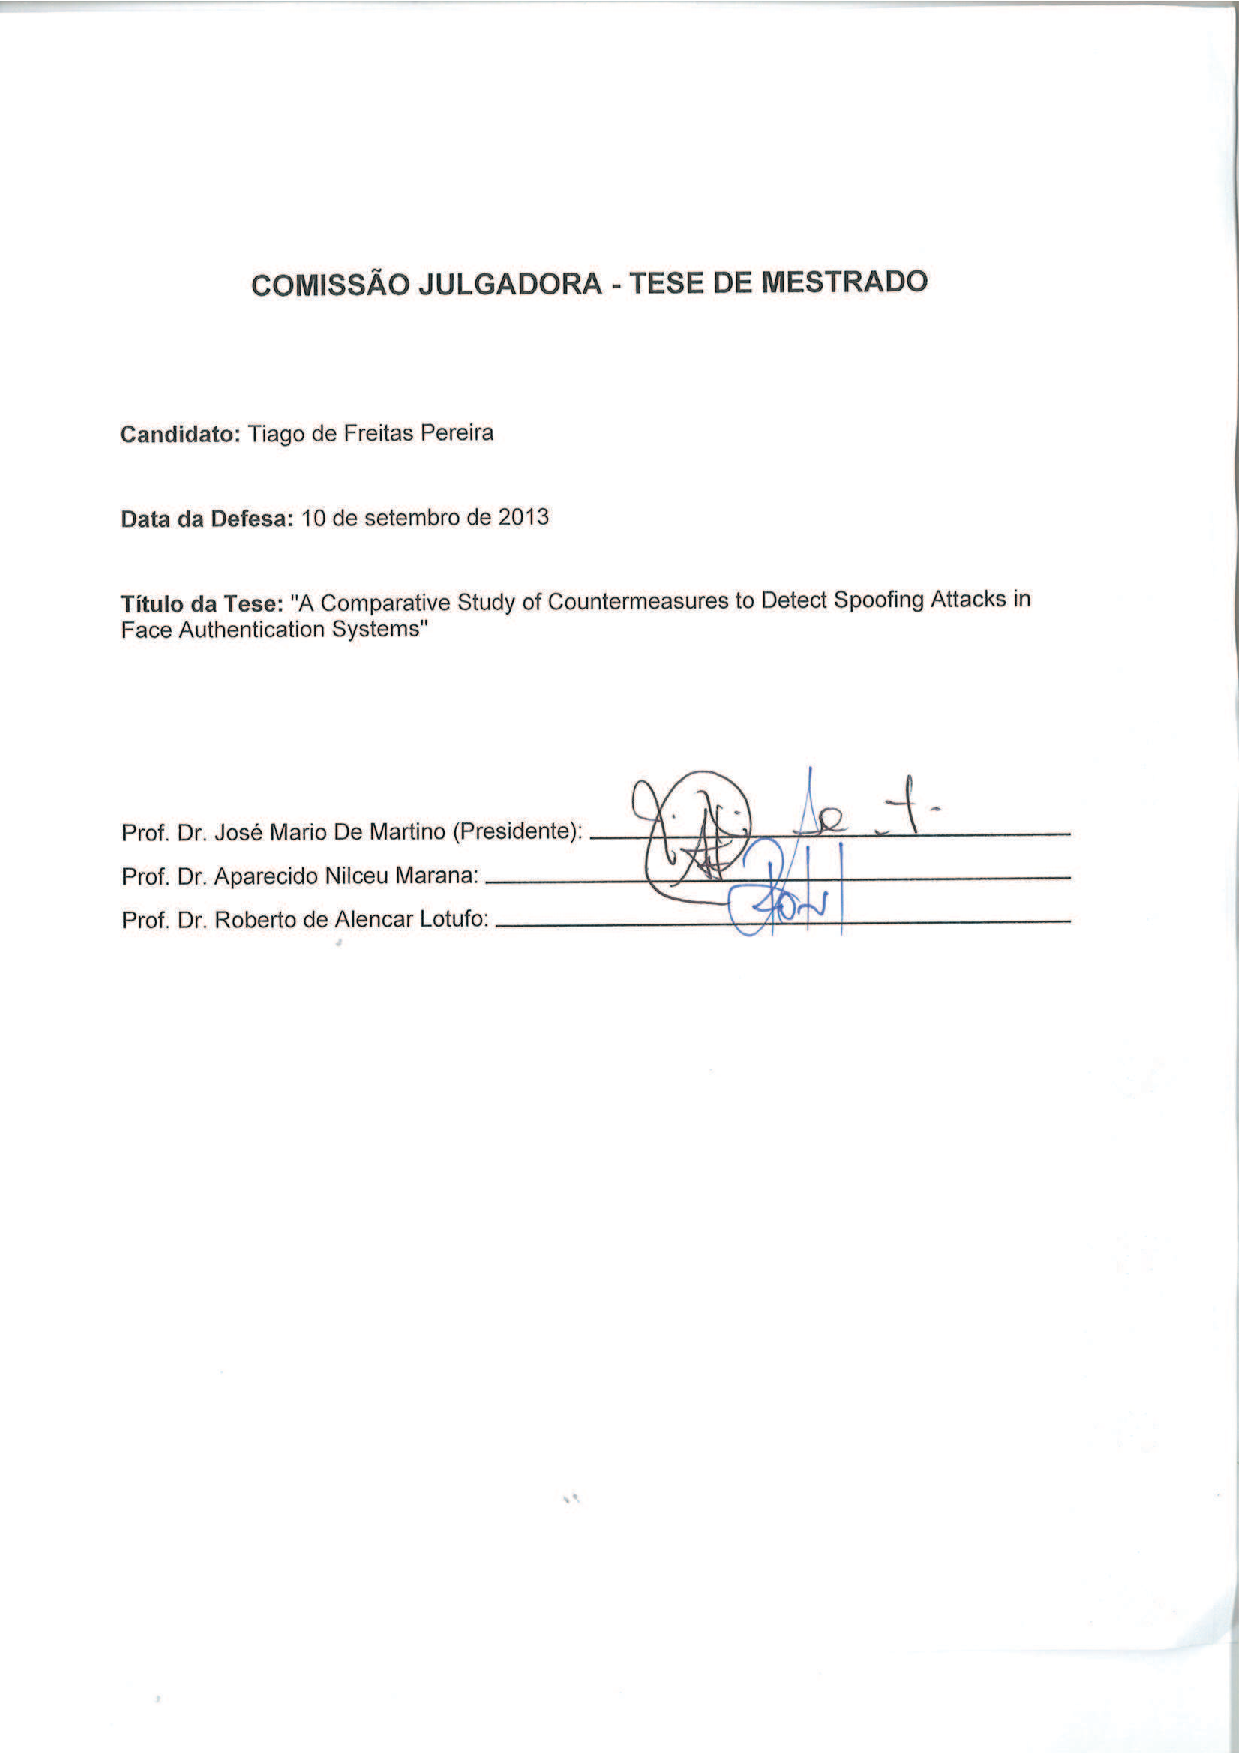
\includepdf[pages=-,pagecommand=\thispagestyle{plain}]{docs/julgamento.pdf}

\newpage %verso em branco
\thispagestyle{empty} %Tirando o numero da primeira p�gina
\addtocounter{page}{-1}
\null
\newpage

